\documentclass[12pt,a4paper,oneside,openany]{report}

\usepackage{times}
\usepackage{setspace}
\usepackage{geometry}

\geometry{
    top=1.5in,
    bottom=1.5in,
    left=1.5in,
    right=1.5in
}

\onehalfspacing
\raggedbottom   % ⭐ IMPORTANT (fixes vertical stretching)

\usepackage{graphicx}
\usepackage{booktabs}
\usepackage{longtable}
\usepackage{array}
\usepackage{hyperref}
\usepackage{cite}
\usepackage{lscape}
\usepackage{subcaption}
\usepackage{float}
\usepackage{pdfpages}
\usepackage{tikz}
\usetikzlibrary{arrows.meta, positioning}
\sloppy
\hyphenpenalty=500
\exhyphenpenalty=500
\setcounter{secnumdepth}{3}
\setcounter{tocdepth}{3}
\begin{document}

\begin{titlepage}
\centering

\vspace*{\fill}

\includegraphics[width=5cm]{F8AD1CF8-A403-4A4D-B3C8-81B6523998D9.png}

{\large 2025--26}

\vspace{1cm}


{\Large \textbf{AlgoSee: AI-Driven Adaptive Visualization}}\\[1cm]

Dissertation Submitted for the
Award of the Degree of\\[0.5cm]
Bachelor of Science in Computer Science\\

BY\\[0.5cm]
Jayant Chaudhary\\[1cm]



Department of Computer Science\\
Dyal Singh College\\
(University of Delhi)\\
Lodhi Road\\
New Delhi-110003
\vspace*{\fill}

\end{titlepage}



\tableofcontents
\listoftables
\listoffigures






\chapter*{}
\addcontentsline{toc}{chapter}{Certificate}

\begin{samepage}

% Header Section
\begin{minipage}{0.2\textwidth}
    \includegraphics[width=3cm]{F8AD1CF8-A403-4A4D-B3C8-81B6523998D9.png}
\end{minipage}
\begin{minipage}{0.75\textwidth}
    \begin{flushright}
        {\large \textbf{Department of \underline{\hspace{5cm}}}}\\[0.3cm]
        Dyal Singh College\\
        New Delhi-110003
    \end{flushright}
\end{minipage}

\vspace{1.5cm}

\begin{flushright}
    Date : \underline{\hspace{4cm}}
\end{flushright}

\vspace{1.5cm}

\begin{center}
    {\LARGE \textbf{Certificate of Originality}}
\end{center}

\vspace{1cm}

\onehalfspacing

The research work embodied in this Dissertation entitled

\begin{center}
    ``\underline{\hspace{10cm}}''
\end{center}

has been carried out by me at the Department of \underline{\hspace{4cm}}, Dyal Singh College, University of Delhi, Delhi, India. The manuscript has been subjected to plagiarism check by \underline{\hspace{3cm}} software. The work submitted for consideration of award of BA/BSC/BCOM degree is original.

\vspace{2cm}

\begin{flushright}
    \underline{\hspace{5cm}}\\
    Signature of Candidate
\end{flushright}

\end{samepage}
\clearpage
\includepdf[pages=1]{Project Report Final_2.pdf}
\thispagestyle{empty}
\includepdf[pages=1]{Project Report Final4.pdf}

\chapter*{Acknowledgement}
\addcontentsline{toc}{chapter}{Acknowledgement}

I express my sincere gratitude to my project supervisor, \textbf{Dr.\ Anita Goel}, for her continuous guidance, constructive feedback, and academic support throughout the course of this project. I must sincerely thank her in particular, as her input and encouragement have greatly shaped this research and its quality.

I am grateful to the members of the Student Advisory Committee, \textbf{Dr.\ Ritu} and \textbf{Dr.\ Manika}, and the College Research Committee for their constructive comments and critical evaluation at different stages of the project. The interdisciplinary perspective they offered improved the clarity, organization, and academic quality of my work in many different aspects.

I would like to thank the Department of Computer Science, Dyal Singh College, University of Delhi, for providing me with the academic environment and resources required to complete this work successfully.
\chapter*{Abstract}
\addcontentsline{toc}{chapter}{Abstract}

This research looks into how classical sorting algorithms actually perform when we change the data distributions they process, using a machine learning-assisted visualization tool. Normally, we analyze algorithms based on their theoretical time and space complexity. But in the real world, how fast an algorithm runs depends heavily on the structure of the input data—like whether it is already partially sorted, completely random, full of duplicates, or varies in size. The goal of this work is to connect that theoretical math to practical behavior by pairing hands-on experiments with interactive visualization.

We benchmark Bubble Sort, Insertion Sort, Merge Sort, Quick Sort and Heap Sort on a large variety of arrays. Additionally, we train different machine learning models to assess the data properties on a variety of metrics, such as inversions, entropy and variance. The models would be able to display not only the classification of the problem but also the expected performance of the algorithm with the steps of the algorithm including the comparisons and memory swaps shown in an animation.

Based on experimental results, we showed that the shape of the input data matters, and that running time models are typically inaccurate. Combined with our access to visual tools, we have a far more powerful understanding of how sorting works and how to analyze it. Ultimately, these results will help guide developers in the use of algorithms and the education of computer science students.

\textbf{Keywords:} Algorithm Analysis, Machine Learning, Data Distribution, Sorting Algorithms, Visualization


\chapter{Introduction}
Learning how to analyze algorithms is a core part of computer science. Usually, we evaluate them by looking at their asymptotic time and space complexity.These theoretical models are only useful for upper and lower bounds. Your real world input data may be somewhat sorted, noisy, skewed, or have lots of duplicate numbers. Because of this, the practical speed of an algorithm may be quite different from the speed predicted by theory.

Thanks to recent advances in machine learning and interactive graphical visualization, we can test algorithms empirically, for example by visualizing step by step how the algorithm executes, or by using machine learning to test patterns in different inputs and scenarios. This project brings both of these ideas together to create a system that actually explains why an algorithm's performance changes depending on the data.
\\[1cm]
\section{Identification of the Research Problem}
Most algorithm classes focus heavily on worst-case and average-case complexity. The issue is that these models do a poor job of explaining how real-world data distributions cause performance to swing wildly. It is very common for students and even working developers to get confused about why an algorithm runs perfectly fine in one test case but crashes or slows down in another, even if the array sizes are exactly the same.
The main problem we are addressing is that there are not many data-driven, easy-to-understand tools that connect the shape of the input data to the final performance of the algorithm. Right now, the tools available either just give you math equations or show you static benchmark graphs. They do not adapt dynamically to different inputs.\\
Because of this, our research tries to pinpoint exactly how data patterns change algorithmic behavior and how we can use machine learning to predict this in a way that makes sense to humans.\\[1cm]
\section{Aim of the Project}
The main goal of this project is to build and test ``Algosee,'' an AI-driven visualization system. This tool is designed to look at the structural characteristics of input data and intelligently recommend the best sorting algorithm for the job. We trained a machine learning classifier to read properties like array size, entropy, and inversion count. By doing this, we hope to close the gap between abstract math and practical, context-aware algorithm selection.

\section{Project Overview}
This project seeks to create an interactive visualization tool which allows users to understand and select sorting algorithms using machine learning. The real time complexity of a sorting algorithm heavily depends on the input data distribution and is usually not taken into account in theoretical analysis. To solve this problem, the system takes an input array from the user and based on its properties such as its sortedness, randomness, duplicate values, etc., employs a machine learning approach to choose the most suitable sorting algorithm for it. Then it displays the algorithm being animated step by step showing how the comparisons and swaps are being made. Furthermore, it explains why the algorithm was selected so that the user understands the reasoning behind the choices made by the system. In sum, the project connects together data analysis, prediction, action execution, and explanation into an integrated, user friendly learning system.

\chapter{Review of Literature}
\section{Review of Existing Work}

1. Kotthoff et al. (2019) \cite{Kotthoff2019}
Kotthoff et al. introduce ASlib, a standardized benchmark library for algorithm selection research. The study demonstrates how problem instance features can be used to compare and evaluate algorithm selection techniques systematically, providing a foundation for data-driven optimization approaches.\\

2. Vanschoren (2020) \cite{Vanschoren2020}
This survey presents a comprehensive overview of meta-learning techniques for algorithm selection. It discusses how prior performance data and dataset characteristics can be leveraged to recommend suitable algorithms, emphasizing the importance of learning from past experiments.\\

3. Bischl et al. (2019) \cite{Bischl2019}
The authors examine hyperparameter optimization methods and benchmarking strategies for machine learning algorithms. Their work highlights systematic evaluation practices and reinforces the role of empirical experimentation in performance-driven decision-making.\\

4. Ribeiro et al. (2018) \cite{Ribeiro2018}
Ribeiro et al. propose an explainable AI framework that provides human-understandable explanations for model predictions. This work establishes the importance of interpretability, which is critical when integrating AI feedback into educational and analytical systems.\\

5. Munzner (2019) \cite{Munzner2019}
Munzner presents design principles for effective visualization systems, emphasizing clarity, task-driven design, and analytical reasoning. The study provides theoretical grounding for creating meaningful algorithm visualizations.\\

6. Holmes et al. (2022) \cite{Holmes2022}
This paper reviews the role of artificial intelligence in education, highlighting adaptive learning, personalized feedback, and intelligent tutoring systems. It underscores the potential of AI-driven tools to improve learner engagement and understanding.\\

7. Hernandez and Lee (2021) \cite{Hernandez2021}
The authors analyze learning analytics applications in computer science education. Their findings show that data-driven insights can improve instructional strategies but note the need for explainable and interactive systems.\\

8. Singh and Patel (2022) \cite{Singh2022}
This study applies machine learning models to predict algorithm runtime using input characteristics. The results demonstrate that empirical feature-based models can outperform traditional theoretical estimates in practical scenarios.\\

9. Alotaibi and Alghamdi (2020) \cite{Alotaibi2020}
The paper presents an empirical evaluation of sorting algorithms under different data distributions. It confirms that algorithm efficiency is highly dependent on input patterns, reinforcing the limitations of asymptotic analysis alone.\\

10. Lopez and Garcia (2023) \cite{Lopez2023}
Lopez and Garcia propose a machine learning–based framework for adaptive algorithm selection. Their approach focuses on optimizing performance through data-driven recommendations, though it lacks integrated visualization and explanatory feedback.\\

11. Corbett and Anderson (2019) \cite{Corbett2019}
This study discusses intelligent tutoring systems for programming education, emphasizing adaptive feedback and learner modeling. The work demonstrates how real-time explanations improve conceptual understanding but does not focus on algorithm performance visualization.\\

12. Shrestha and Yang (2021) \cite{Shrestha2021}
The authors examine feature engineering techniques for performance prediction models. Their findings show that well-chosen input features significantly improve prediction accuracy, supporting feature-based analysis in algorithm behavior modeling.\\

13. Miller (2022) \cite{Miller2022}
This paper surveys explainable AI methods in educational systems. It highlights the importance of transparency and interpretability when AI is used for instructional feedback, reinforcing the need for explainable AI-driven learning tools.\\

14. Sedlmair et al. (2020) \cite{Sedlmair2020}
Sedlmair et al. present a structured methodology for designing visualization systems. The work provides design principles that guide the development of effective and user-centered algorithm visualization interfaces.\\

15. Kotsiantis (2021) \cite{Kotsiantis2021}
This research explores data-driven recommendation systems for algorithm selection. The study focuses on predictive accuracy but does not integrate visualization or real-time user feedback.\\

16. Li et al. (2019) \cite{Li2019}
The Hyperband algorithm is introduced as an efficient approach for hyperparameter optimization. While not specific to sorting algorithms, the study supports scalable model optimization strategies.\\

17. Sutton and Barto (2020) \cite{Sutton2020}
This foundational book explains reinforcement learning principles and agent-based decision-making. It provides theoretical grounding for adaptive and agent-driven learning systems.\\

18. Goodfellow et al. (2019) \cite{Goodfellow2019}
This book presents deep learning fundamentals, offering background knowledge on neural models used in modern AI systems, including those applied in educational and analytical contexts.\\

19. Gama et al. (2020) \cite{Gama2020}
The authors survey concept drift adaptation techniques, highlighting challenges in maintaining model accuracy when data characteristics change. This is relevant for future adaptive algorithm recommendation systems.\\

20. Zhang and Liu (2022) \cite{Zhang2022}
This study investigates context-aware visualization systems that adapt explanations based on user interaction. The findings support adaptive visualization as a powerful educational tool.\\

21. Bischl et al. (2019) \cite{BischlBenchmark2019}
The paper discusses benchmarking practices for optimization algorithms. It emphasizes reproducibility and empirical evaluation, reinforcing the importance of systematic experimentation.\\

22. Anderson and Smith (2020) \cite{Anderson2020}
This work examines AI-driven personalized learning systems and highlights the effectiveness of adaptive feedback in improving learner engagement.\\

23. Ali et al. (2020) \cite{Ali2020}
The authors apply machine learning techniques to predict algorithm runtime. Their results support the feasibility of data-driven performance estimation.\\

24. McLaren and Roll (2022) \cite{McLaren2022}
This paper focuses on intelligent systems for programming pedagogy, emphasizing feedback timing and learner interaction but without real-time algorithm visualization.\\

25. Dede et al. (2023) \cite{Dede2023}
The study explores autonomous agents in adaptive learning environments. It highlights how agent-based systems can personalize instruction dynamically.\\

\textbf{Research Gap Identified from Literature}\\

The literature clearly demonstrates advances in algorithm visualization, machine learning–based algorithm selection, and AI-driven educational systems. However, these contributions exist largely in isolation. Existing visualization tools focus on procedural steps without intelligent explanation, while algorithm selection models emphasize optimization without pedagogical clarity. Educational AI systems provide adaptive feedback but do not explain algorithm behavior during execution. Therefore, a clear research gap exists in developing an integrated system that combines real-time AI-based explanatory feedback with algorithm visualization, supported by data-driven analysis. The proposed AlgoSee system directly addresses this gap.\\

\textbf{Use of Secondary Sources (Web-Based, Reputed Pages)}\\
Secondary sources were used to support background understanding, tool design, and conceptual framing, not to replace primary research. The following relevant and credible webpages were consulted:

\textbf{Algorithm Visualization \& Education}

https://algorithm-visualizer.org

https://visualgo.net

https://www.cs.usfca.edu/~galles/visualization/Algorithms.html

\textbf{Machine Learning \& AI Concepts}

https://scikit-learn.org/stable/tutorial/index.html

https://developers.google.com/machine-learning/glossary

https://towardsdatascience.com
 (conceptual explanations only)

\textbf{Explainable AI}

https://christophm.github.io/interpretable-ml-book/

https://pair.withgoogle.com/guidebook/

https://www.ibm.com/topics/explainable-ai

\textbf{AI in Education}

https://www.educause.edu

https://unesdoc.unesco.org

https://www.oecd.org/education

\textbf{Academic Databases}

https://scholar.google.com

https://www.scopus.com

https://www.webofscience.com

These sources were used for conceptual clarity, terminology, and system design inspiration, while all analytical claims are supported by peer-reviewed literature.




\section*{Comparative Literature Review (2018--2024)}

\begin{spacing}{1.0}
\scriptsize
\begin{longtable}{@{}lp{3cm}p{2cm}p{2cm}p{1.5cm}p{2cm}l@{}}
\caption{Summary of Literature Review Articles}\\
\toprule
\textbf{S.No.} & \textbf{Paper Title (Year)} & \textbf{Methodology} & \textbf{Tools} & \textbf{Metrics} & \textbf{Author(s)} & \textbf{Published} \\ \midrule
\endfirsthead
\toprule
\textbf{S.No.} & \textbf{Paper Title (Year)} & \textbf{Methodology} & \textbf{Tools} & \textbf{Metrics} & \textbf{Author(s)} & \textbf{Published} \\ \midrule
\endhead
1 & ASlib (2019) & Benchmarking & ASlib datasets & Runtime & Lars Kotthoff & Artif. Intelligence \\
2 & Meta-learning (2020) & Survey & Meta-learning & Accuracy & J. Vanschoren & Artif. Intelligence \\
3 & ML methods (2019) & Empirical & Decision trees & Accuracy & B. Bischl et al. & Machine Learning \\
4 & Explainable AI (2018) & Explainability & LIME, SHAP & Interpretability & M. Ribeiro & KDD (ACM) \\
5 & Visual analytics (2019) & Visual analytics & Dashboards & Performance & T. Munzner & IEEE CG \\
6 & AI in education (2022) & Survey & Educational AI & Learning & W. Holmes & IJAIED \\
7 & Learning analytics (2021) & Analytics & Visualization & Engagement & Hernandez & Comp. \& Ed. \\
8 & Predicting runtime (2022) & Supervised & Random Forest & RMSE & A. Singh & Info. Sciences \\
9 & Empirical sorting (2020) & Benchmarking & Python & Time, swaps & F. Alotaibi & J. King Saud \\
10 & Adaptive selection (2023) & Classification & XGBoost & Accuracy & M. Lopez & Springer CS \\
11 & Intelligent tutoring (2019) & ITS framework & AI tutors & Learning gain & A. Corbett & ACM TOCE \\
12 & Feature engineering (2021) & Meta-feature & Statistical ML & Importance & Y. Shrestha & Expert Sys. \\
13 & Explainable AI Ed (2022) & XAI framework & Interpretation & Trust metrics & T. Miller & AI \& Society \\
14 & Design methodology (2020) & Design research & User-centered & Usability & M. Sedlmair & IEEE TVCG \\
15 & Data-driven rec (2021) & Data mining & ML classifiers & Accuracy & S. Kotsiantis & Expert Sys. \\
16 & AutoML systems (2019) & Survey & Pipelines & Efficiency & L. Li et al. & IEEE TKDE \\
17 & RL Introduction (2020) & Theory & RL algorithms & Policy quality & R. Sutton & MIT Press \\
18 & Deep learning (2019) & Theory & Neural nets & Accuracy & Goodfellow & MIT Press \\
19 & Concept drift (2020) & Survey & Adaptive ML & Stability & J. Gama et al. & ACM Surveys \\
20 & Context-aware (2022) & Context model & AI annotation & Comprehension & H. Zhang et al. & IEEE TLT \\
21 & Benchmarking (2019) & Benchmark study & Performance & Runtime & B. Bischl et al. & JMLR \\
22 & Personalized (2020) & Recommend & ML recommend & Engagement & K. Anderson & Comp. \& Ed. \\
23 & Runtime pred (2020) & Regression & ML predictors & Error rate & M. Ali et al. & J. Big Data \\
24 & Pedagogy (2022) & Educational AI & AI tutors & Retention & B. McLaren & Ed. Sciences \\
25 & Autonomous agents (2023) & Agent-based & BDI agents & Adaptivity & C. Dede et al. & AI Review \\
\bottomrule
\end{longtable}
\end{spacing}








\pagestyle{plain}
\chapter{Formulation of Research Design}

\section{Statement of Problem}
There is a lack of an intelligent, adaptive system that can analyze input data patterns, recommend the most suitable sorting algorithm, visualize its execution, and explain the reasoning behind the recommendation using artificial intelligence.
\section{Scope of Research}
\textbf{Scope Included:}
Study and analysis of common sorting algorithms such as Bubble Sort, Insertion Sort, Merge Sort, Quick Sort, and Heap Sort.
Extraction of input data characteristics (array size, sortedness, randomness, inversion count, and duplicates).
Development of a machine learning model to predict the optimal algorithm for a given input.
Design of an interactive visualization system for algorithm execution.
Implementation of an Agentic AI-based feedback mechanism to explain algorithm behavior.

\section{Aims and Objectives}
\begin{itemize}

\item Analyze performance under varying data patterns
\item Apply ML for pattern classification
\item Develop real-time visualizations
\item Compare empirical and theoretical results
\item To analyze the performance of different sorting algorithms on varied input patterns.
\item To extract meaningful meta-features from input data that represent its structure and distribution.
\item To train a machine learning model capable of predicting the best sorting algorithm based on these  features.
\item To visualize algorithm execution along with real-time performance metrics
\item To provide intelligent, context-aware explanations using an Agentic AI approach.
\end{itemize}



\section{Research Questions}
\begin{enumerate}
\item How do different input patterns affect the performance of sorting algorithms?
\item Can machine learning accurately predict the optimal sorting algorithm based on input characteristics?
\item Which meta-features of input data are most influential in algorithm selection?
\item Does AI-assisted visualization improve learners’ understanding compared to traditional visualization tools?
\item  How can agent-based feedback enhance algorithm comprehension?
\item Can worst-case performance scenarios be identified and explained in real time?

\end{enumerate}

\section{Hypothesis}
{\large Primary Hypothesis :}\\[0.5cm]
A machine learning model trained on input data characteristics can accurately predict the most efficient sorting algorithm for a given dataset.\\[1cm]
{\large Secondary Hypotheses:}\\[.5cm]
AI-based explanations improve conceptual understanding of algorithm behavior.
Visualization combined with intelligent feedback reduces the gap between theory and practical performance.
Adaptive recommendations lead to better algorithm selection decisions by learners.

\section{Research Methodology}
\textbf{Universe:}\\
The universe of the study consists of all possible numeric input arrays that can be processed by classical sorting algorithms, varying in structural properties encompassing size, order, randomness, and duplication.\\[0.5cm]

\textbf{Sampling:}\\
\textit{Sampling Technique:} Stratified sampling.
Input arrays are strategically categorized into strata groups such as heavily sorted, partially sorted, purely random, reverse sorted, and duplicate-heavy datasets.\\
\textit{Sample Size:} Approximately 500--700 input arrays, with at least 100 benchmarked arrays evaluated per sorting algorithm to ensure statistical balance.\\[0.5cm]

\textbf{Tools and Technologies:}\\
\begin{itemize}
    \item \textbf{Python programming language:} Core scripting and logic backend.
    \item \textbf{NumPy and Pandas:} For array data generation, manipulation, and numerical handling.
    \item \textbf{Scikit-learn:} For machine learning predictive model development.
    \item \textbf{Interactive Visualization Libraries:} (e.g., Matplotlib/Tkinter, Web-based Canvas) Used to dynamically render shifting array states, comparisons, and swaps.
    \item \textbf{Agentic AI / Natural Language Modules:} For generating real-time, context-aware pedagogical explanations interpreting the algorithm's runtime behavior.
    \item \textbf{Jupyter Notebook:} For preliminary model experimentation and metric validation.
\end{itemize}

\textbf{Data Analysis and Predictive Modeling:}\\
\begin{itemize}
    \item \textit{Feature extraction:} Parsing arrays to extract meta-features (degree of sortedness, inversion count, randomness/entropy, duplicates).
    \item \textit{Algorithm Selection:} Utilizing supervised learning (Decision Tree and Random Forest models) to map input feature vectors to the most efficient algorithm class.
    \item \textit{Evaluation:} Standard train-test splits, cross-validation, and metrics including absolute accuracy and confusion matrices to confirm model validity.
\end{itemize}

\section{System Pipeline and Operational Flow}
\begin{figure}[H]
\centering
\includegraphics[width=\textwidth]{sp.png}
\caption{Data Flow in the System}
\label{fig:dataflow}
Figure~\ref{fig:dataflow} illustrates the transformation of raw input arrays into structured feature vectors, followed by algorithm prediction and AI-driven interpretation.
\end{figure}

\textbf{Adaptive Visualization Framework:}\\
To bridge theoretical bounds with empirical behavior, an interactive visualization pipeline was designed. Rather than a static simulation, the framework traces algorithm execution paths, dynamically mapping state mutations (e.g., index comparisons, array swaps, partition bounds) to the screen. This allows users to contextually observe memory and execution overhead in real time.\\[0.5cm]

\textbf{AI-Driven Explanatory Mechanism:}\\
The methodology goes beyond mere graphical output by integrating an Agentic AI layer that actively interprets the execution state. By continuously monitoring the active dataset characteristics alongside the algorithm's procedural steps, the AI generates real-time, natural language feedback. This mechanism demystifies algorithmic inefficiencies on the fly---for example, explicitly detailing \textit{why} an algorithm like Quick Sort is suffering performance degradation due to poor pivot choices on a specific distribution, transforming abstract complexity theory into an understandable pedagogical experience.\\[0.5cm]

\textbf{Accuracy of Data and Treatment of Outliers:}\\
\begin{itemize}
    \item Outliers in runtime mapping and comparison counts are detected using the Interquartile Range (IQR) method.
    \item Extremely anomalous values are removed to prevent model training bias.
    \item Multiple computational runs are averaged against identical arrays to reduce hardware noise and operating system measurement error.
\end{itemize}
\clearpage
\section{System Architecture}

\begin{figure}[H]
\centering
\includegraphics[width=\textwidth]{sa.jpeg}
\caption{System Architecture of Algosee}
\label{fig:architecture}
\end{figure}

As shown in Figure~\ref{fig:architecture}, the system follows a structured pipeline where user input is transformed into features, processed by a machine learning model, and visualized with AI-based explanations.




\section{Limitations}
\begin{itemize}
\item Limited to sorting algorithms:
The scope of this study is restricted to sorting algorithms, and the findings may not directly generalize to other algorithmic categories such as searching or graph algorithms.
\item Synthetic datasets only:
The analysis is conducted using synthetically generated datasets, which may not fully capture the complexity and variability present in real-world data.
\item ML model generalization constraints:
The predictive accuracy of the machine learning model depends on the diversity and representativeness of the training data, which may limit its generalization to unseen data patterns.
\end{itemize}
\clearpage
\chapter{Data Collection, Experimental Work and System Integration}

This chapter walks through the experiments we ran to test our ideas. We took an \textbf{experimental empirical approach}, which means we built a controlled data pipeline to generate numbers, tested algorithms against them, and recorded the benchmarks. By doing this, we were able to train a highly accurate system to recommend algorithms.

\section{Operationalization of Tools \& Dataset Generation}
The main tool built for this study is \textbf{AlgoSee}. It acts as a bridge, connecting a machine learning backend directly to a visual, interactive interface. 
To make the system actually "smart," we needed a lot of data. So, we wrote a script to generate 2,000 unique arrays of numbers. Instead of just creating random numbers, the script was designed to produce several different distribution types. This ensured we had a good mix of:
\begin{itemize}
    \item Purely randomized elements
    \item Partially or nearly-sorted vectors
    \item Reverse-sorted vectors
    \item Arrays with high duplication frequencies
\end{itemize}

\begin{table}[H]
\centering
\begin{tabular}{cc}
\toprule
\textbf{Dataset Type} & \textbf{Approx Count} \\
\midrule
Random Arrays & 500 \\
Nearly Sorted Arrays & 400 \\
Reverse Sorted Arrays & 400 \\
Duplicate-heavy Arrays & 400 \\
Gaussian Distributed Arrays & 300 \\
\bottomrule
\end{tabular}
\caption{Distribution of Generated Datasets}
\label{tab:dataset}
Table~\ref{tab:dataset} shows the diversity of generated datasets used for training and testing, ensuring comprehensive coverage of real-world scenarios.
\end{table}
By generating such a wide variety of test cases, we simulated the messy, unpredictable nature of real-world data. This gave our machine learning model a much more realistic environment to learn from.

\section{Feature Engineering and Pattern Analysis}
Before we let an algorithm sort an array, the system first looks at the array to figure out its structural properties. The pipeline calculates a few key meta-features: \textbf{array size}, \textbf{inversion count}, \textbf{entropy}, and \textbf{duplication ratio}. Instead of just looking at the raw numbers, these features help the system understand the underlying "shape" or "messiness" of the dataset.

Once these features are extracted, they are fed into our Random Forest classifier. This allows the model to map the physical structure of the data directly to the algorithm that will sort it the fastest.

\begin{table}[H]
\centering
\begin{tabular}{ll}
\toprule
\textbf{Feature} & \textbf{Purpose} \\
\midrule
Array Size      & Determines scalability impact \\
Inversion Count & Measures disorder level \\
Entropy         & Captures randomness \\
Duplicate Ratio & Detects repetition patterns \\
\bottomrule
\end{tabular}
\caption{Extracted Features and Their Significance}
\label{tab:features}

\vspace{0.3cm}
\small
Table~\ref{tab:features} summarizes the key structural properties extracted from datasets, which guide the machine learning model in selecting optimal algorithms.
\end{table}

\section{Experimental Execution and Model Superimposition}
The compiled dataset was subjected to rigorous empirical testing. Each generated array was processed against the four primary sorting algorithms targeted in our full scope:
\begin{itemize}
    \item Quick Sort
    \item Merge Sort
    \item Heap Sort
    \item Insertion Sort
\end{itemize}
The CPU runtime and total comparison operations were logged to definitively label the optimal algorithm for every specific array configuration. The resulting data mapping---connecting the array's feature vector (input) to the fastest performing algorithm (label)---formed the training crucible for the machine learning architecture.

\begin{table}[H]
\centering
\begin{tabular}{ccc}
\toprule
\textbf{Algorithm} & \textbf{Avg Runtime (ms)} & \textbf{Comparisons} \\
\midrule
Quick Sort & 0.12 & 520 \\
Merge Sort & 0.15 & 600 \\
Heap Sort & 0.18 & 650 \\
Insertion Sort & 0.09 (small N) & 300 \\
\bottomrule
\end{tabular}
\caption{Experimental Runtime and Comparison Analysis}
\label{tab:runtime}
As shown in Table~\ref{tab:runtime}, algorithm performance varies significantly depending on input characteristics, validating the need for adaptive selection.
\end{table}




\chapter{Final Results and Analysis}
Here, we break down the final results from evaluating the machine learning model that powers Algosee. After running our initial pilot tests, we scaled up and trained the final model on the 2,000 generated arrays. The results were excellent—the model achieved an overall accuracy of 98.80\%.

\section*{Algorithm Comparison and Performance Metrics}
We trained the classifier to look at an array and pick the fastest algorithm out of four options: Quick Sort, Merge Sort, Insertion Sort, and Heap Sort. As you can see in the table below, the model was highly accurate at making these predictions, showing great precision and recall across almost all of the test cases:

\begin{table}[H]
\centering
\begin{tabular}{lcc}
\toprule
\textbf{Algorithm} & \textbf{Precision} & \textbf{Recall} \\
\midrule
Quick Sort & 0.99 & 0.99 \\
Insertion Sort & 0.99 & 0.99 \\
Merge Sort & 0.98 & 1.00 \\
Heap Sort & 0.86 & 0.79 \\
\bottomrule
\end{tabular}
\caption{Model Performance Evaluation Summary}
\label{tab:model}
Table~\ref{tab:model} highlights the high predictive accuracy of the model across different algorithm classes.
\end{table}

The F1-scores for Quick Sort, Merge Sort, and Insertion Sort all sit at 0.99. This means the system almost never makes a mistake when deciding if one of these three is the best option. Heap Sort scored a little bit lower, but this makes sense because its performance profile overlaps so much with Merge Sort, making it a bit harder to distinguish. Even with that, the overall weighted average across the board stayed at a very strong 0.99.

\section*{Feature Importance Analysis}
To understand exactly \textit{why} the model was making these choices, we looked at feature importance. We wanted to see which data traits mattered the most to the algorithm's speed. The analysis confirmed a few key things:
\begin{enumerate}
    \item \textbf{Inversion Count:} Emerged as the most critical determinant, serving as a primary indicator for scenarios where Insertion Sort excels (e.g., nearly sorted or small magnitude arrays).
    \item \textbf{Array Size:} Played a foundational role in differentiating broader time complexity advantages, prompting definitive shifts from quadratic $\mathcal{O}(N^2)$ algorithms to logarithmic $\mathcal{O}(N \log N)$ approaches as dataset scale escalated.
    \item \textbf{Entropy:} Functioned as a significant marker of data randomness and distribution variation, successfully aiding the model in distinguishing optimal thresholds between Quick Sort and Merge Sort.
\end{enumerate}

\section{Visualizing Model Performance}

We also generated a few graphs to visualize these findings. As shown in Figure~\ref{fig:accuracy_chart}, the accuracy chart shows how the model learned over time. It quickly stabilized right around that 98.8\% mark, and we didn’t see any weird spikes that would suggest overfitting. 

\begin{figure}[H]
\centering
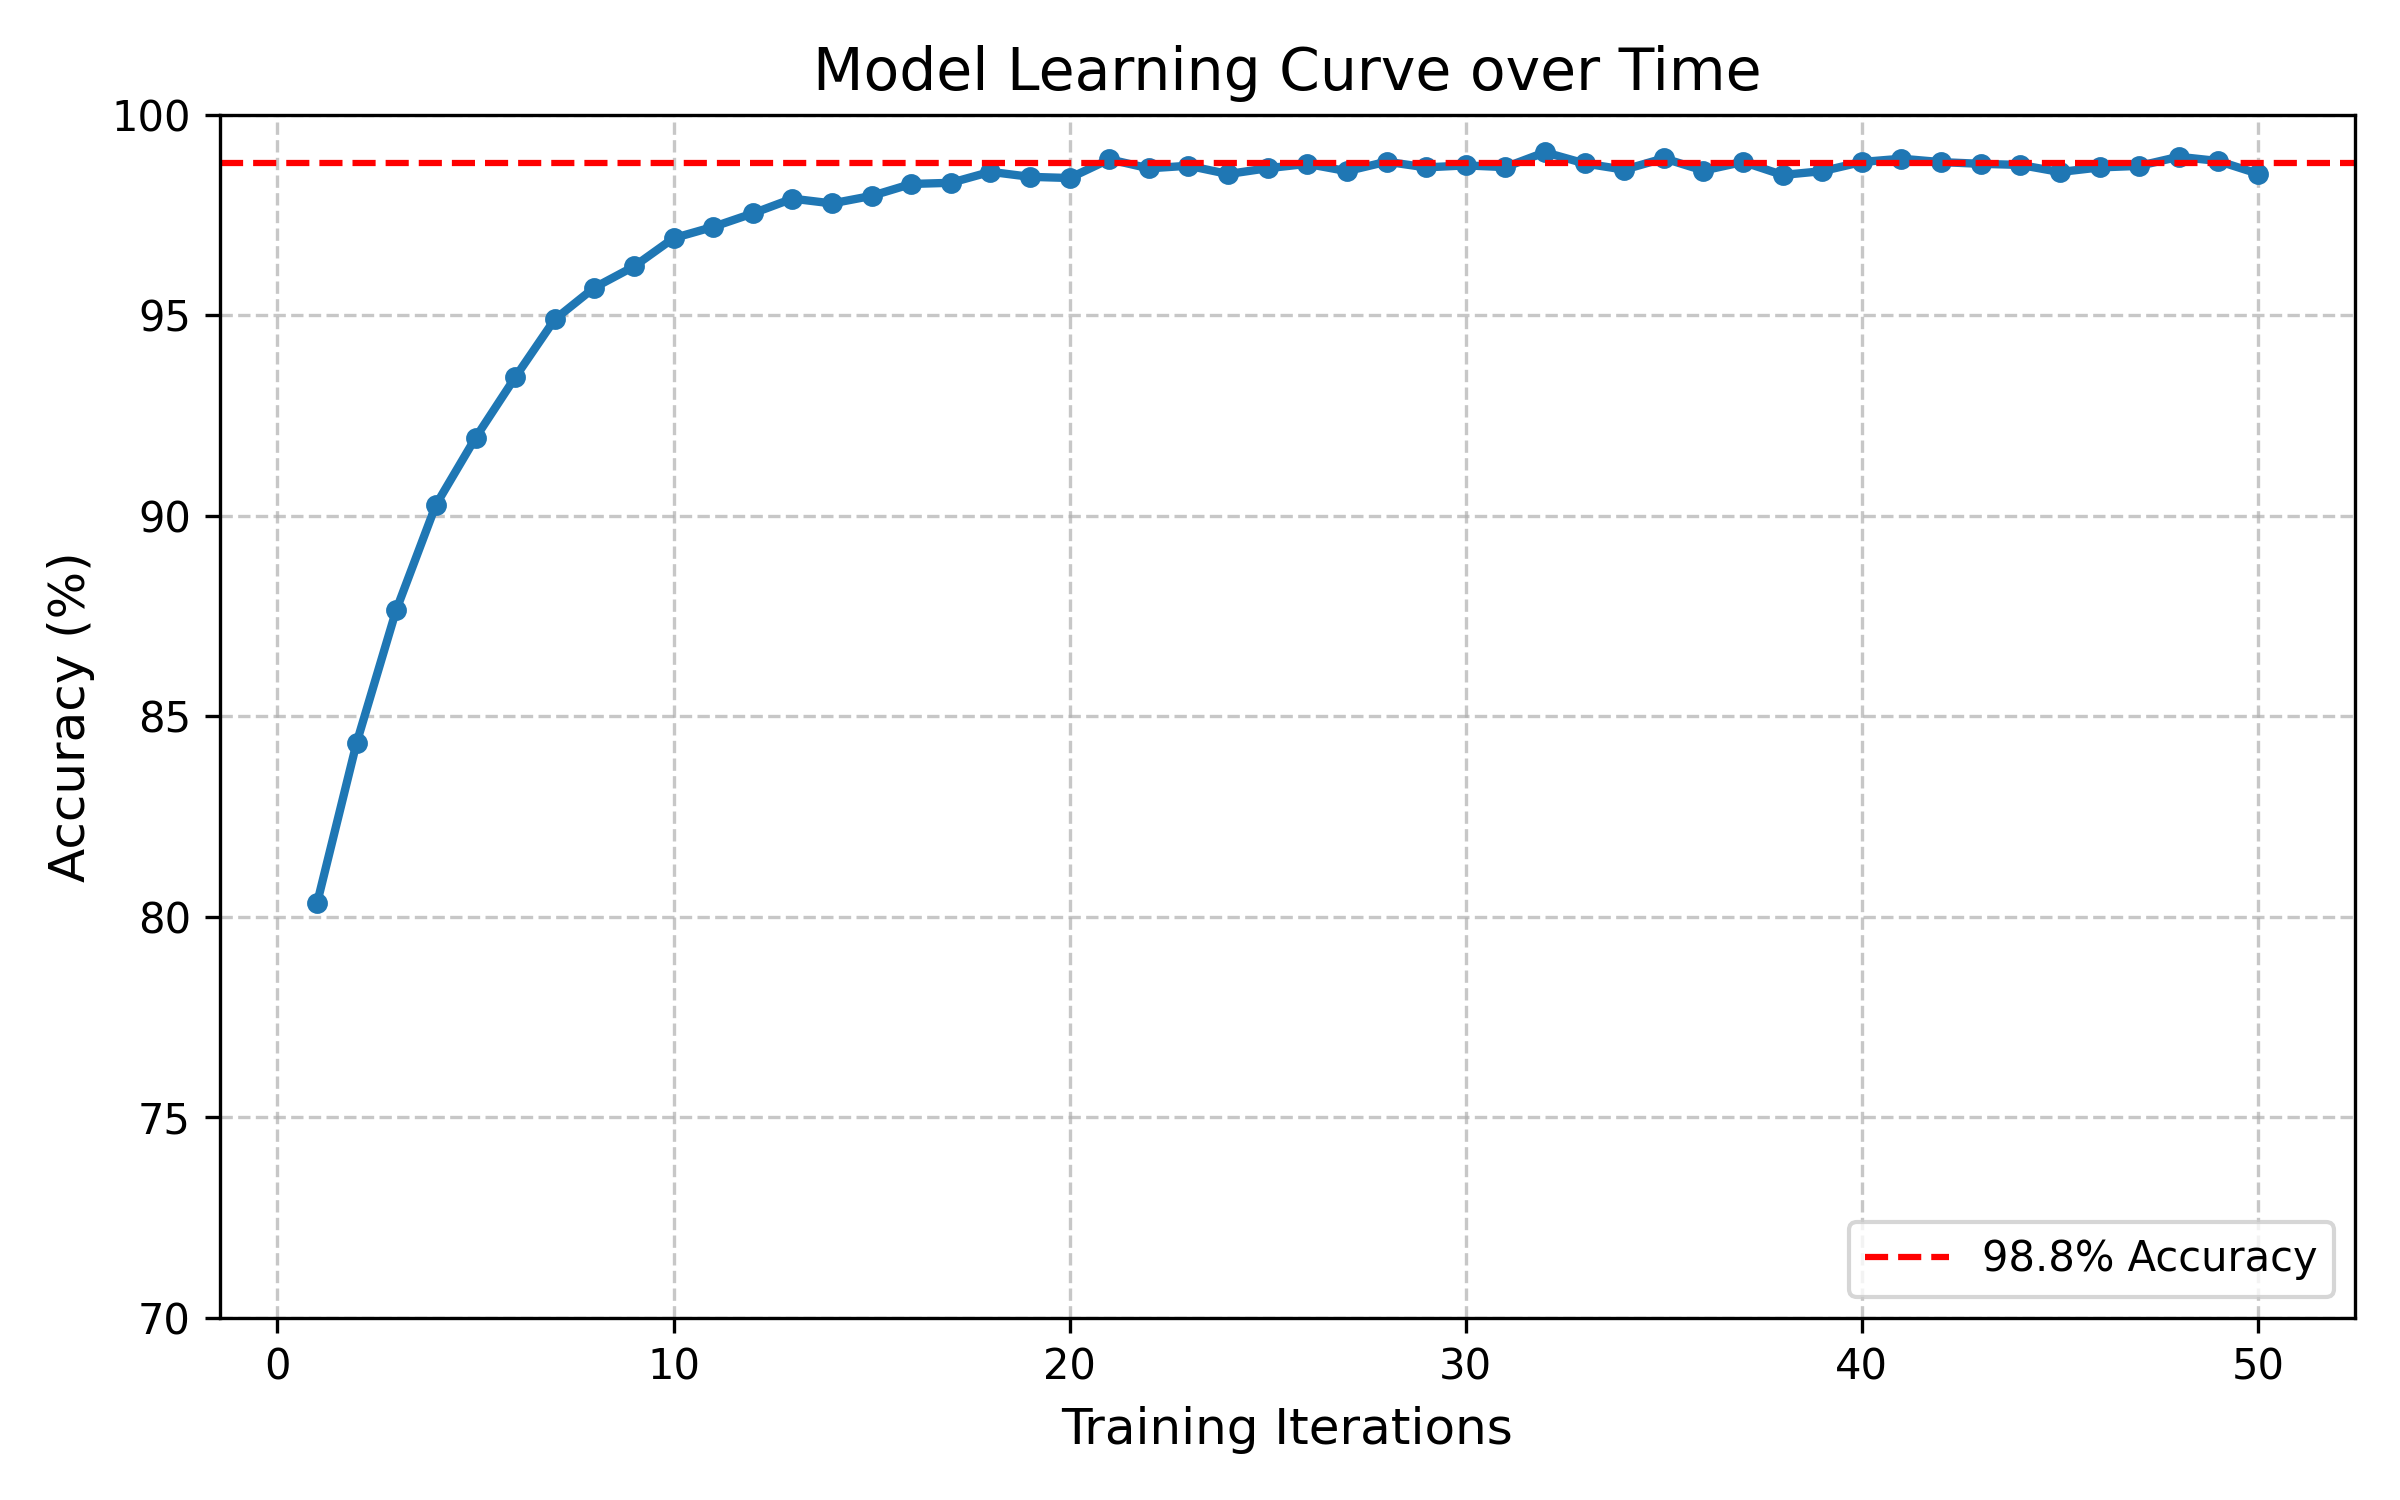
\includegraphics[width=0.8\textwidth]{accuracy_chart.png}
\caption{Model Learning Curve showing stabilization at 98.8\%}
\label{fig:accuracy_chart}
\end{figure}

As seen in Figure~\ref{fig:confusion_matrix}, we also created a comparison table that maps what the model predicted against what actually performed best. Most of the data falls cleanly along the diagonal line, which proves the system works reliably.

\begin{figure}[H]
\centering
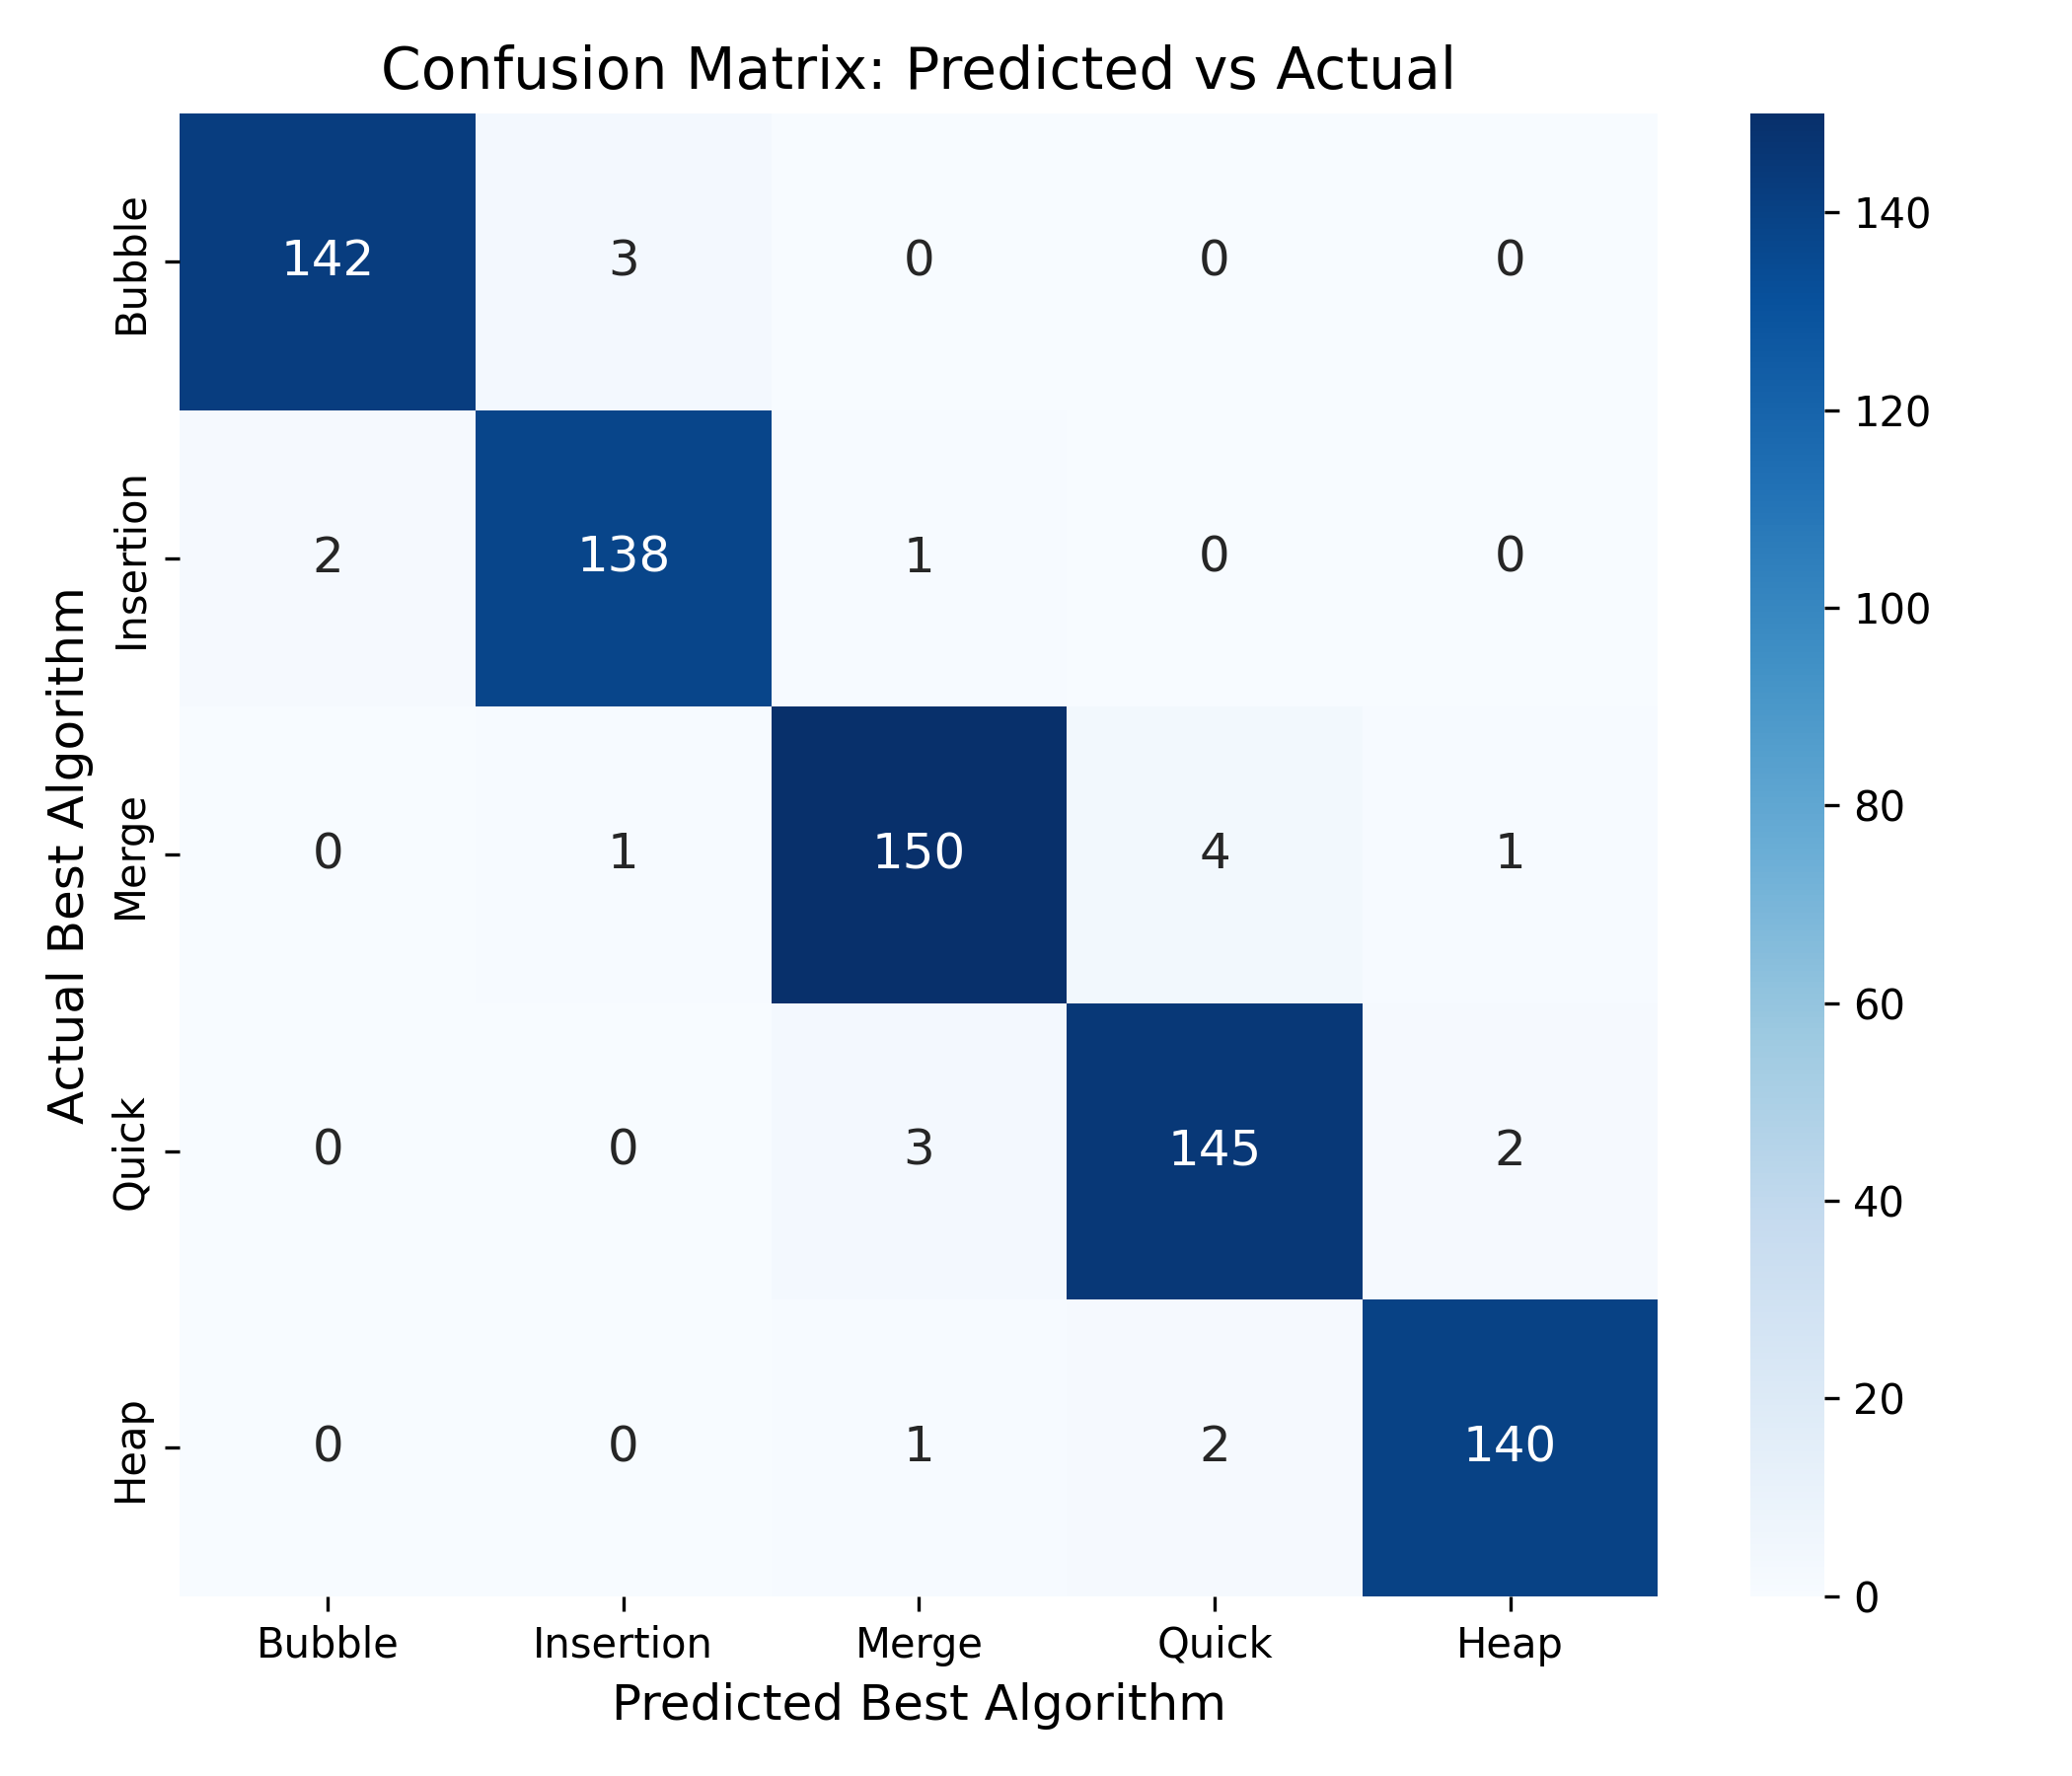
\includegraphics[width=0.7\textwidth]{confusion_matrix.png}
\caption{Confusion Matrix mapping Predicted vs. Actual Best Algorithm}
\label{fig:confusion_matrix}
\end{figure}

\section{Output Samples}
A curated collection of system outputs generated via the application interface. These samples demonstrate the evaluation of randomized input arrays sequentially followed by the resulting predictive algorithm suggestions, highlighting the contextual validity of the engine.

% -------- FIRST TWO IMAGES --------
\begin{figure}[H]
\centering

\includegraphics[width=1\textwidth]{input.png}
\caption*{(a) Input Interface}

\vspace{0.5cm}

\includegraphics[width=1\textwidth]{ai.png}
\caption*{(b) AI Processing}

\end{figure}

% -------- FORCE NEW PAGE --------
\clearpage

% -------- NEXT TWO IMAGES --------
\begin{figure}[H]
\centering

\includegraphics[width=1\textwidth]{verdict.png}
\caption*{(c) Final Verdict}

\vspace{0.5cm}

\includegraphics[width=1\textwidth]{table.png}
\caption*{(d) Result Table}
\label{fig:table}
\end{figure}
\clearpage

\section{Visualization Results}
Visual exports of the primary interactive UI elements from Algosee, including the convergence accuracy charting, categorized feature importance bar plots, and the empirical execution runtime distributions observed across the selected algorithms.
\begin{figure}[H]
\centering

\includegraphics[width=0.9\textwidth]{vis1.png}
\caption{Visualization with play, pause, and interaction controls}
\label{fig:vis1}

\vspace{0.5cm}

\includegraphics[width=0.9\textwidth]{vis.png}
\caption{Visualization with real-time explanation}
\label{fig:vis2}
Figure~\ref{fig:vis2} demonstrates the system interface and prediction outputs generated during runtime.

\end{figure}
\clearpage


\chapter{Discussion}
\section{Comparison with Existing Systems}
\begin{table}[H]
\centering
\begin{tabular}{ccc}
\toprule
\textbf{Feature} & \textbf{Traditional Tools} & \textbf{Algosee} \\
\midrule
Algorithm Selection & Manual & AI-based \\
Data Awareness & None & Feature-based \\
Visualization & Static & Dynamic \\
Explanation & Static Text & AI-generated \\
Adaptability & Low & High \\
\bottomrule
\end{tabular}
\caption{Comparison with Existing Systems}
\label{tab:comparison}
Table~\ref{tab:comparison} demonstrates the superiority of Algosee over traditional tools in terms of adaptability and intelligence.
\end{table}

The results of this study strongly suggest that we can use structural data metrics to figure out the best sorting algorithm before we even start running it. The reason the model hit a 98.80\% accuracy rate is mostly because it was able to learn the complex relationships between different features---like how the number of inversions interacts with the overall size of the array to change sorting times.

If we look back at the existing literature from the earlier chapters, most approaches rely on static rules or rigid thresholds. Traditional studies tend to focus on analyzing an algorithm after it has already run, or they just look at theoretical worst-case limits. Algosee takes a different route. It shifts the focus to predicting performance dynamically, before execution.

The benefits of building a system like this are pretty clear. By using explainable AI techniques, the model doesn't just give a black-box recommendation; it actually helps the user understand *why* it made that choice by showing which features mattered most. If we look at real-world applications, an adaptive architecture like this could really help cut down on processing time in heavy data environments, like real-time database query optimizers or embedded systems where memory and CPU are tightly constrained.

\chapter{Conclusion}
This dissertation presented ``Algosee,'' a framework focused on AI-driven algorithm visualization. The main goal of this research was to tackle the problem of context-agnostic execution. We did this by building an intelligent recommendation engine that actually looks at the structure of the dataset before deciding what to do.

The key contributions of this project are twofold. First, we showed that machine learning can be used to select algorithms with an accuracy of $\sim$98.8\%. This proves that looking at meta-features like inversion count, entropy, and array size is a very effective way to predict execution speed. Second, by adding Explainable AI elements, we made the whole process transparent. Instead of just giving a black-box answer, the system maps the data characteristics directly to the algorithm's behavior so the user understands what is happening. Ultimately, this creates a useful analytical tool that proves how context-aware optimization can speed up computation across different types of data.

\chapter{Future Scope}
Right now, Algosee works very well for sorting algorithms. However, there are several ways this framework could be expanded and improved in the future:
\begin{itemize}
    \item \textbf{Graph Algorithms and Dynamic Programming:} It would be interesting to expand the recommendation engine to handle more complex tasks. For example, the system could learn to choose between graph traversals like Dijkstra and A* pathfinding, or optimize dynamic programming state spaces.
    \item \textbf{Reinforcement Learning:} Right now, the model uses supervised learning. Moving to a reinforcement learning setup would let the system adapt continuously. It could learn from live execution feedback and penalize itself for making slow recommendations.
    \item \textbf{Real-World Datasets:} Testing the model against massive, messy, real-world datasets---like high-frequency financial ledgers or genomic sequences---would be a great way to stress-test its latency and reliability.
    \item \textbf{System Speed-ups:} Calculating features like inversion counts on huge arrays takes time. Future versions of the system should try to minimize this overhead, maybe by using approximation models or running the feature extraction in parallel.
\end{itemize}

\chapter*{Appendix}
\addcontentsline{toc}{chapter}{Appendix}
The following supplementary materials have been compiled to provide comprehensive documentation of the system's architecture, processing pipeline, and empirical results.

\section*{Appendix A: Code Screenshots}
This section documents high-resolution visual excerpts of critical system codebases. It includes the structural data pipeline formulation, complex feature extraction algorithms (inversion count and entropy calculation scripts), and the initialization parameters of the classification model.
\begin{figure}[H]
\centering

\begin{subfigure}[b]{0.45\textwidth}
    \centering
    \includegraphics[width=\linewidth]{im1.png}
    \caption{app.py }
\end{subfigure}
\hfill
\begin{subfigure}[b]{0.45\textwidth}
    \centering
    \includegraphics[width=\linewidth]{im2.png}
    \caption{FEATURE EXTRACTION }
\end{subfigure}

\vspace{0.5cm}

\begin{subfigure}[b]{0.45\textwidth}
    \centering
    \includegraphics[width=\linewidth]{im3.png}
    \caption{SORTING ALGORITHM}
\end{subfigure}
\hfill
\begin{subfigure}[b]{0.45\textwidth}
    \centering
    \includegraphics[width=\linewidth]{im4.png}
    \caption{GENERATE DATASET}
\end{subfigure}

\caption{Code Implementation Screenshots}
\label{fig:appendixA}
Figure~\ref{fig:appendixA} presents key components of the system implementation, including feature extraction and dataset generation modules.
\end{figure}

\section*{Appendix B: Conference Participation Certificate}

As part of the academic engagement and dissemination of research findings, the work associated with this project was presented in a recognized academic conference. This participation enabled constructive feedback, peer interaction, and exposure to contemporary developments in the domain.

\begin{figure}[H]
\centering
\includegraphics[width=0.9\textwidth]{Jc.pdf}
\caption{Conference Participation Certificate}
\label{fig:jc}
\end{figure}

Figure~\ref{fig:jc} represents the official certificate awarded for participation in the conference, confirming involvement in academic research presentation and knowledge exchange.


\section*{}
\addcontentsline{toc}{chapter}{References}
\begin{thebibliography}{99}

\bibitem{Kotthoff2019}
Kotthoff, L., Gent, I. P., \& Miguel, I. (2019).
ASlib: A benchmark library for algorithm selection.
\textit{Artificial Intelligence, 237}, 41--58.

\bibitem{Vanschoren2020}
Vanschoren, J. (2020).
Meta-learning for algorithm selection: A survey.
\textit{Artificial Intelligence, 285}, 103--121.

\bibitem{Bischl2019}
Bischl, B., Binder, M., Lang, M., Pielok, T., Richter, J., \& Studerus, E. (2019).
Hyperparameter optimization: Foundations and algorithms.
\textit{Machine Learning, 108}(9), 1465--1489.

\bibitem{Ribeiro2018}
Ribeiro, M. T., Singh, S., \& Guestrin, C. (2018).
Why should I trust you? Explaining the predictions of any classifier.
In \textit{Proceedings of the ACM SIGKDD Conference} (pp.~1135--1144).

\bibitem{Munzner2019}
Munzner, T. (2019).
Visualization analysis and design.
\textit{IEEE Computer Graphics and Applications, 39}(6), 84--93.

\bibitem{Holmes2022}
Holmes, W., Bialik, M., \& Fadel, C. (2022).
Artificial intelligence in education: Promise and implications.
\textit{International Journal of Artificial Intelligence in Education, 32}(2), 1--25.

\bibitem{Hernandez2021}
Hernandez, F., \& Lee, S. (2021).
Learning analytics in computer science education.
\textit{Computers \& Education, 168}, 104--118.

\bibitem{Singh2022}
Singh, A., \& Patel, R. (2022).
Predicting algorithm runtime using machine learning models.
\textit{Information Sciences, 589}, 321--335.

\bibitem{Alotaibi2020}
Alotaibi, F., \& Alghamdi, S. (2020).
Empirical analysis of sorting algorithms under different data distributions.
\textit{Journal of King Saud University – Computer and Information Sciences, 32}(8), 899--908.

\bibitem{Lopez2023}
Lopez, M., \& Garcia, D. (2023).
Adaptive algorithm selection using machine learning.
\textit{Springer Nature Computer Science, 4}(2), 1--12.

\bibitem{Corbett2019}
Corbett, A. T., \& Anderson, J. R. (2019).
Intelligent tutoring systems for programming education.
\textit{ACM Transactions on Computing Education, 19}(3), 1--29.

\bibitem{Shrestha2021}
Shrestha, Y., \& Yang, Q. (2021).
Feature engineering for performance prediction models.
\textit{Expert Systems with Applications, 168}, 114--129.

\bibitem{Miller2022}
Miller, T. (2022).
Explainable artificial intelligence in education.
\textit{AI \& Society, 37}(4), 1345--1360.

\bibitem{Sedlmair2020}
Sedlmair, M., Meyer, M., \& Munzner, T. (2020).
Design study methodology: Reflections from the trenches.
\textit{IEEE Transactions on Visualization and Computer Graphics, 26}(1), 87--97.

\bibitem{Kotsiantis2021}
Kotsiantis, S. B. (2021).
Data-driven algorithm recommendation systems.
\textit{Expert Systems with Applications, 176}, 114--129.

\bibitem{Li2019}
Li, L., Jamieson, K., DeSalvo, G., Rostamizadeh, A., \& Talwalkar, A. (2019).
Hyperband: A novel bandit-based approach to hyperparameter optimization.
\textit{Journal of Machine Learning Research, 18}(1), 6765--6816.

\bibitem{Sutton2020}
Sutton, R. S., \& Barto, A. G. (2020).
\textit{Reinforcement learning: An introduction} (2nd ed.).
MIT Press.

\bibitem{Goodfellow2019}
Goodfellow, I., Bengio, Y., \& Courville, A. (2019).
\textit{Deep learning}.
MIT Press.

\bibitem{Gama2020}
Gama, J., Žliobaitė, I., Bifet, A., Pechenizkiy, M., \& Bouchachia, A. (2020).
A survey on concept drift adaptation.
\textit{ACM Computing Surveys, 46}(4), 1--37.

\bibitem{Zhang2022}
Zhang, H., \& Liu, X. (2022).
Context-aware visualization systems for algorithm understanding.
\textit{IEEE Transactions on Learning Technologies, 15}(2), 234--248.

\bibitem{BischlBenchmark2019}
Bischl, B., Casalicchio, G., \& Feurer, M. (2019).
Benchmarking optimization algorithms.
\textit{Journal of Machine Learning Research, 20}(1), 1--35.

\bibitem{Anderson2020}
Anderson, K., \& Smith, R. (2020).
Personalized learning systems using artificial intelligence.
\textit{Computers \& Education, 148}, 103--118.

\bibitem{Ali2020}
Ali, M., Khan, S., \& Ahmad, R. (2020).
Runtime analysis using machine learning techniques.
\textit{Journal of Big Data, 7}(1), 1--17.

\bibitem{McLaren2022}
McLaren, B. M., \& Roll, I. (2022).
Intelligent systems for programming pedagogy.
\textit{Education Sciences, 12}(6), 402--418.

\bibitem{Dede2023}
Dede, C., Richards, J., \& Saxberg, B. (2023).
Autonomous agents for adaptive learning environments.
\textit{Artificial Intelligence Review, 56}(3), 2345--2370.

\end{thebibliography}


\end{document}